\section{Phase 3 - Classification Analysis}

\subsection{Classification Pipeline}

Per the requirements, for each classifier grid search to find the hyper parameter is needed. To improve code readability and functionality, the design of pipeline is as follows.

For each classifier, define a parameter grid, which is a python dictionary that contains the parameter candidates. The pipeline function takes the classifier object and the parameter candidates as inputs. For pipeline function, grid search with 5 \textbf{stratified cross validation} is executed, and the scorer for every classifier is set to accuracy.

After the hyper parameter for the classifier is found, the model with the hyper parameter is used to to make predictions. Thanks to\\ \texttt{sklearn.model\_selection.GridSearchCV}'s optimization for automation, best estimator is stored to prevent further training of the data.

Using best estimator of the grid search, predictions are retrieved on test set. An object of \texttt{ClassifierMetrics} is created. This class is a self defined class to estimate the performance of the classifier. The metrics include confusion\_matrix, precision, recall, specificity, f1\_score and roc\_auc based on probability.

After all performance metrics are calculated, the classifier's True Positive Rate vs False Positive Rate is plotted. A classifier's pipeline comes to an end here. After all classifier finished training and running, a master table and subplot of all classifiers performance will be displayed. 

\subsection{Pre-pruning Decision Tree}

Two classifiers are considered for Decision Tree: pre-pruning and post-pruning. For pre-pruning, parameter candidates are shown in table~\ref{tab:parameters-pre-dt}. To retrieve the best result while reduce the cost of training, the parameters are selected to be start, middle and end of a range of possible candidates. 

\begin{table}[h]
\centering
\begin{tabular}{|l|r|}
\hline
\textbf{Parameter}         & \textbf{Values}                   \\ \hline
max\_depth         & 1, 4, 10                          \\ \hline
min\_samples\_split & 2, 5, 10                          \\ \hline
min\_samples\_leaf  & 1, 4                              \\ \hline
max\_features      & 1, 5, 10, sqrt, log2              \\ \hline
splitter           & best, random                      \\ \hline
criterion          & gini, entropy                     \\ \hline
\end{tabular}
\caption{Parameter Candidates for Pre-pruning Decision Tree}
\label{tab:parameters-pre-dt}
\end{table}

The best parameters for this classifier are displayed to the console:

\begin{verbatim}
Best parameters set found:
{'criterion': 'entropy', 'max_depth': 10, 'max_features': 10,
'min_samples_leaf': 1, 'min_samples_split': 2, 'splitter': 'best'}
\end{verbatim}

Figure~\ref{fig:roc-dt-pre} shows the ROC curve of pre-pruning decision tree, the model obtained an AUC of \textbf{0.79}.

\begin{figure}
    \centering
    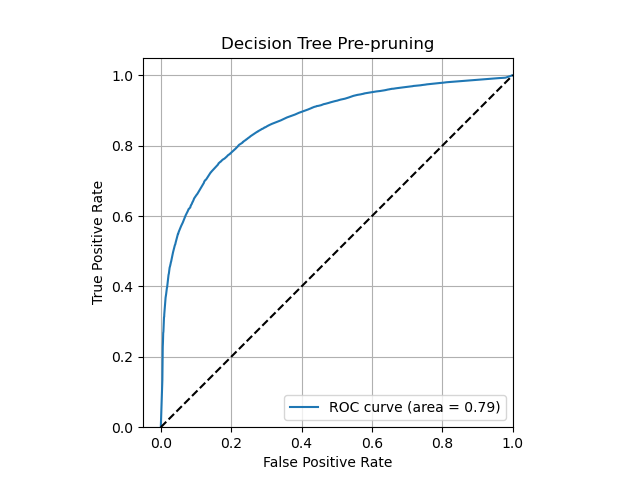
\includegraphics[width=1\linewidth]{docs//assets/individual_roc_curve_Decision Tree Pre-pruning.png}
    \caption{ROC Curve for Pre-pruning Decision Tree}
    \label{fig:roc-dt-pre}
\end{figure}

Table~\ref{tab:pre-dt} is the metrics for pre-pruning tree. From the recall and specificity, the observation is that pre-pruning decision tree performs better on positive class.

\begin{table}
\centering
\begin{tabular}{|c|c|c|c|c|c|c}
\hline
\textbf{Precision} & \textbf{Recall} & \textbf{Specificity} & \textbf{F1 Score} & \textbf{AUC} & \textbf{Confusion Matrix} \\
\hline
0.804 & 0.770 & 0.812 & 0.786 & 0.791 & $\left(\begin{array}{cc} 13032 & 3020 \\ 3699 & 12352 \end{array}\right)$ \\ 
\hline
\end{tabular}
\caption{Metrics for Pre-pruning Decision Tree}
\label{tab:pre-dt}
\end{table}

\subsection{Post-pruning Decision Tree}

For Post-pruning Decision Tree Classifier, the grid search is set to the \texttt{ccp\_alpha} parameter. Table~\ref{tab:parameters-dt-post} displays the candidates for \texttt{ccp\_alpha}. \texttt{ccp} is short for cost complexity pruning, which indicates the aggressiveness of pruning. Greater values of ccp\_alpha increase the number of nodes pruned.

\begin{table}[h]
\centering
\begin{tabular}{|l|r|}
\hline
\textbf{Parameter} & \textbf{Values}            \\ \hline
ccp\_alpha         & 0.0, 0.01, 0.1, 0.2, 0.5, 1.0 \\ \hline
\end{tabular}
\caption{Parameter Candidates for Post-pruning Decision Tree}
\label{tab:parameters-dt-post}
\end{table}
The best parameters for this classifier are displayed to the console:

\begin{verbatim}
Best parameters set found:
{'ccp_alpha': 0.01}
\end{verbatim}

Figure~\ref{fig:roc-dt-post} shows the ROC curve of post-pruning decision tree, the model obtained an AUC of \textbf{0.78}, less effective than pre-pruning tree.

\begin{figure}
    \centering
    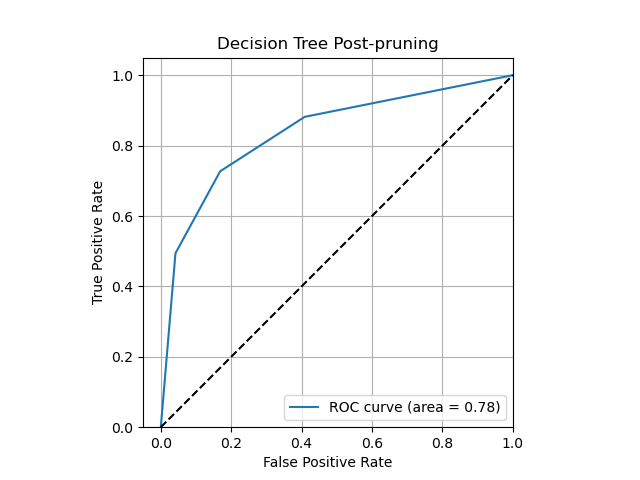
\includegraphics[width=1\linewidth]{docs//assets/individual_roc_curve_Decision Tree Post-pruning.png}
    \caption{ROC Curve for Post-pruning Decision Tree}
    \label{fig:roc-dt-post}
\end{figure}

Table~\ref{tab:post-dt} is the metrics for post-pruning tree. The specificity is higher than the pre-pruning, meaning that false alarm rate is lowered. However, the AUC is decreased compared to the pre-pruning tree.

\begin{table}
\centering
\begin{tabular}{|c|c|c|c|c|c|c}
\hline
\textbf{Precision} & \textbf{Recall} & \textbf{Specificity} & \textbf{F1 Score} & \textbf{AUC} & \textbf{Confusion Matrix} \\
\hline
0.812 & 0.727 & 0.831 & 0.767 & 0.779 & $\left(\begin{array}{cc} 13345 & 2707 \\ 4381 & 11670 \end{array}\right)$ \\ 
\hline
\end{tabular}
\caption{Metrics for Post-pruning Decision Tree}
\label{tab:post-dt}
\end{table}

Additionally, more ccp\_alpha values are being considered to estimate the best value. Figure~\ref{fig:ccp} shows the procedure of the estimation. In order to prevent over-fitting and inaccuracy, the first alpha where train sets and test sets meet should be chose for optimal value, which is 0.01, the same as the result in the grid search.

\begin{figure}
    \centering
    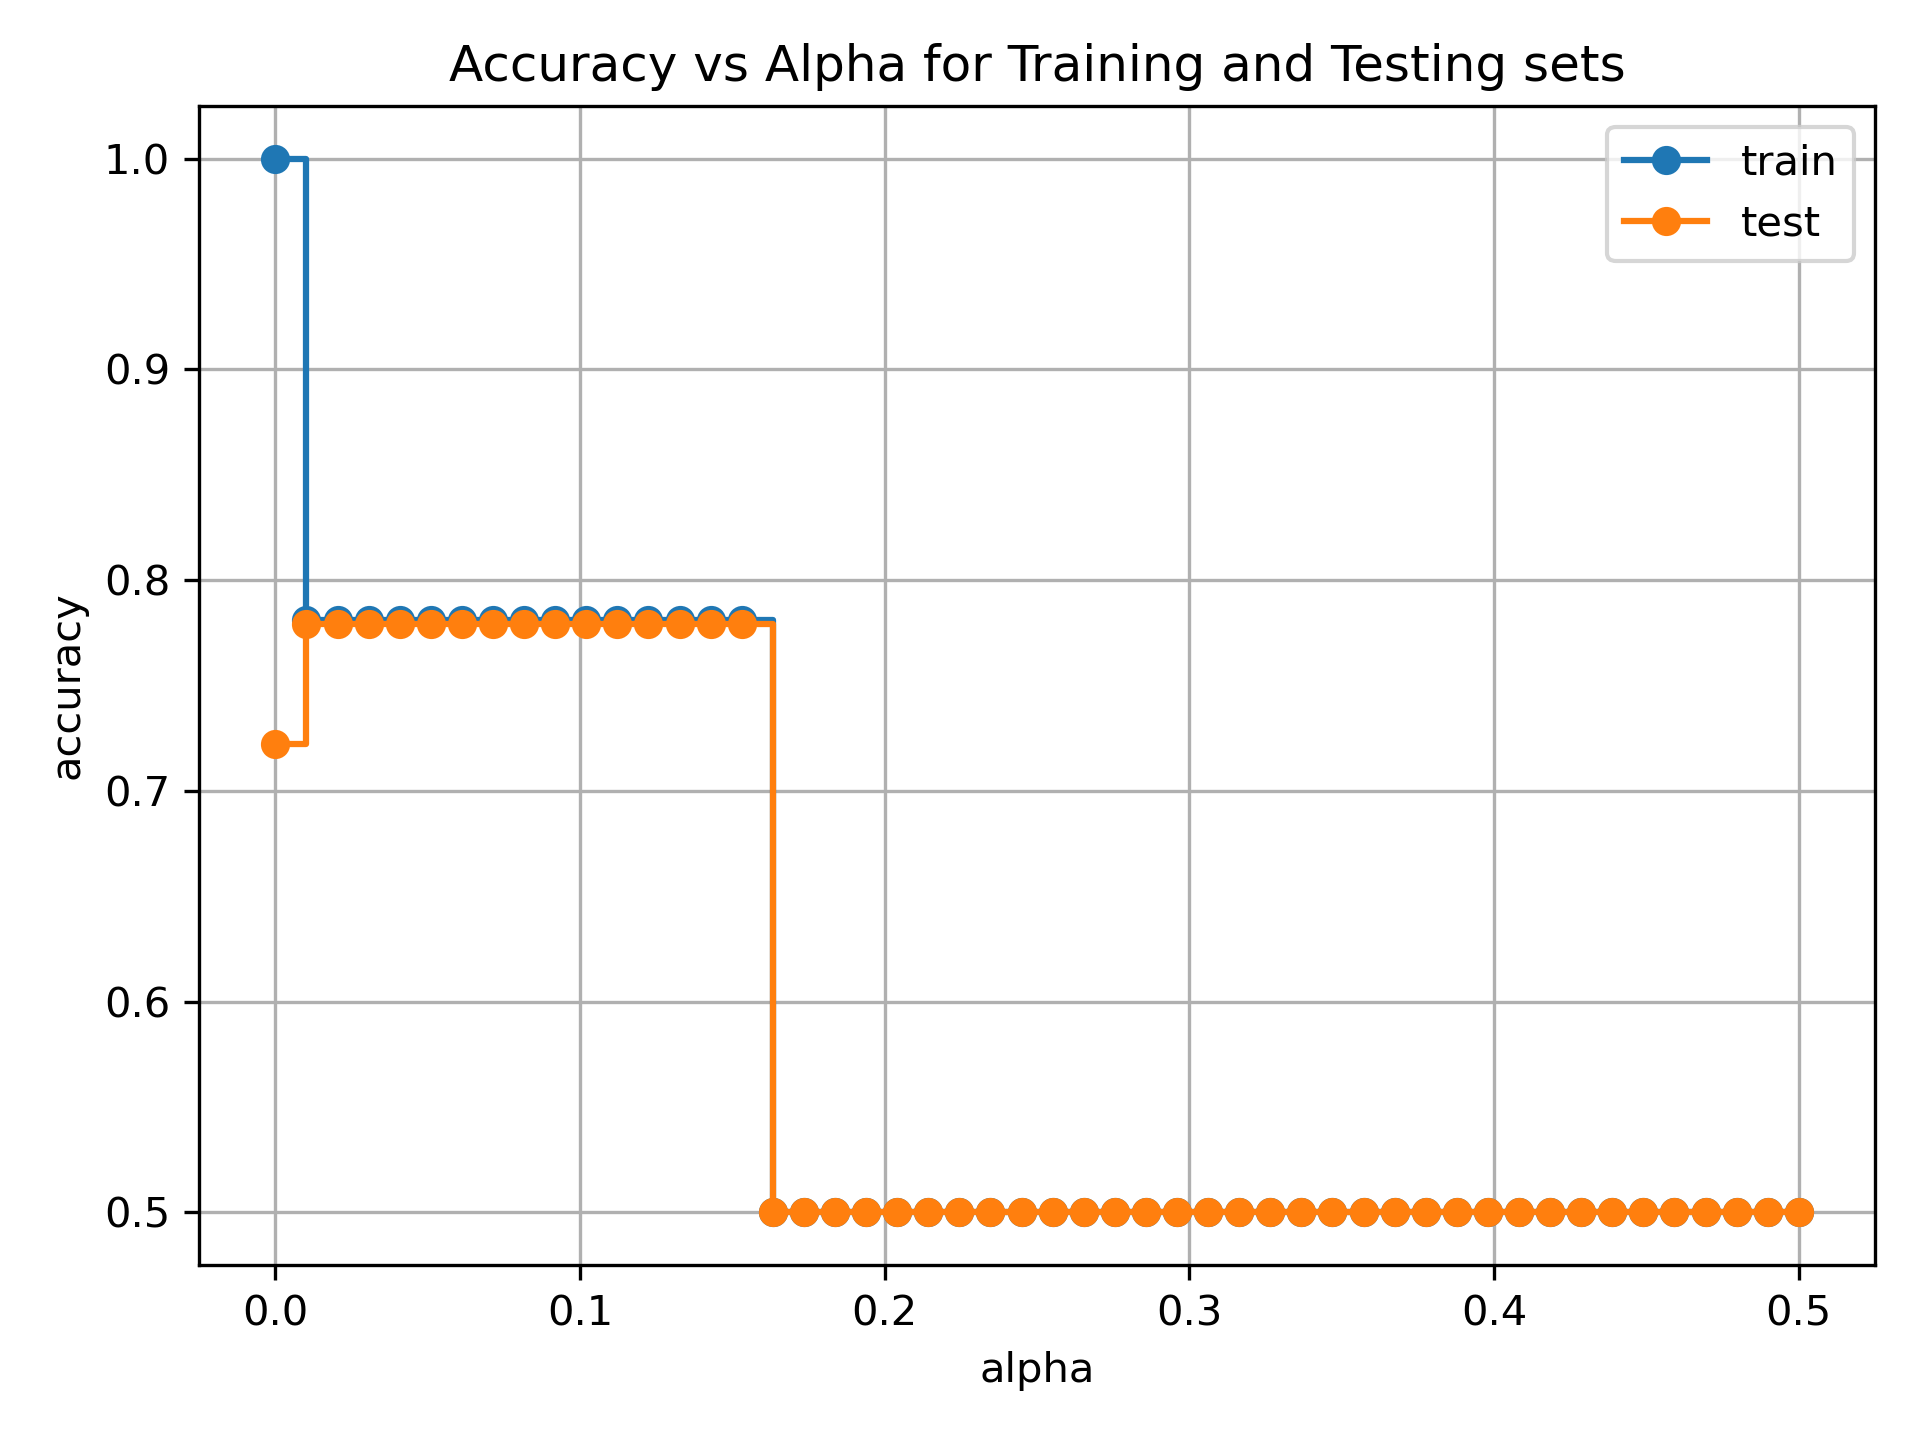
\includegraphics[width=1\linewidth]{docs//assets/accuracy_vs_alpha.png}
    \caption{Accuracy vs. ccp\_alpha}
    \label{fig:ccp}
\end{figure}


\subsection{Logistic Regression}

For Logistic Regression Classifier, the grid search is set to various parameters. Table~\ref{tab:parameters-logreg} displays the candidates. \texttt{C} is the inverse of regularization strength.\textit{A high value of C tells the model to give high weight to the training data, and a lower weight to the complexity penalty.}\cite{stack_overflow_c_parameter}. For l2 penalty, the only solver supported is \texttt{lbfgs}.

\begin{table}[h]
\centering
\begin{tabular}{|l|r|}
\hline
\textbf{Parameter} & \textbf{Values}            \\ \hline
penalty            & l2                         \\ \hline
C                  & 0.1, 1, 10                \\ \hline
solver             & lbfgs                      \\ \hline
max\_iter          & 100, 200, 300, 400, 500    \\ \hline
\end{tabular}
\caption{Parameter Candidates for Logistic Regression Model}
\label{tab:parameters-logreg}
\end{table}

The best parameters for this classifier are displayed to the console. A large C is preferred, indicating that the training data is reliable, thanks to stratified target and cross validation.

\begin{verbatim}
Best parameters set found:
{'C': 10, 'max_iter': 100, 'penalty': 'l2', 'solver': 'lbfgs'}
\end{verbatim}

Figure~\ref{fig:roc-lr} shows the ROC curve of logoistic regression classifier, the model obtained an AUC of \textbf{0.77}, less effective than decision tree.

\begin{figure}
    \centering
    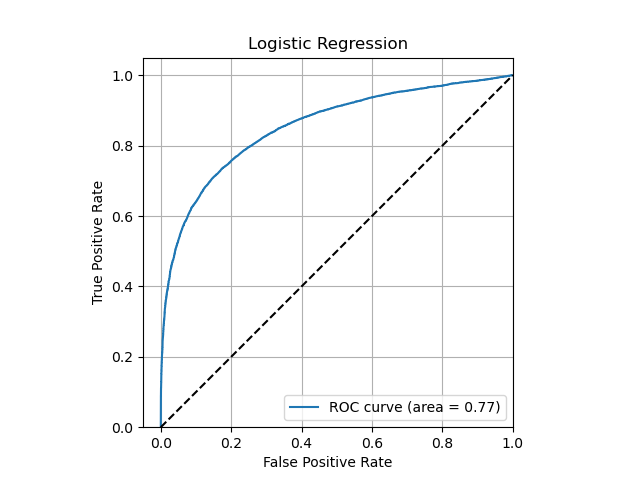
\includegraphics[width=1\linewidth]{docs//assets/individual_roc_curve_Logistic Regression.png}
    \caption{ROC Curve for Logistic Regression}
    \label{fig:roc-lr}
\end{figure}

Table~\ref{tab:lr} is the metrics for logistic regression. The specificity is significantly higher than recall. The logistic regression classifier might do a better job in avoid false alarm, in this case, the low \texttt{installCount} apps, but might not have much confidence in the result that tells the user their apps' \texttt{installCount} is high.

\begin{table}
\centering
\begin{tabular}{|c|c|c|c|c|c|c}
\hline
\textbf{Precision} & \textbf{Recall} & \textbf{Specificity} & \textbf{F1 Score} & \textbf{AUC} & \textbf{Confusion Matrix} \\
\hline
0.864 & 0.641 & 0.899 & 0.736 & 0.770 & $\left(\begin{array}{cc} 14437 & 1615 \\ 5756 & 10295 \end{array}\right)$ \\ 
\hline
\end{tabular}
\caption{Metrics for Logistic Regression}
\label{tab:lr}
\end{table}

\subsection{K-Nearest Neighbors}

For K-Nearest Neighbors (KNN) classification, the grid search is set to find the best k and the best way to estimate the distance. Table~\ref{tab:parameters-knn} displays the parameter candidates.

\begin{table}[h]
\centering
\begin{tabular}{|l|r|}
\hline
\textbf{Parameter} & \textbf{Values}                                \\ \hline
n\_neighbors       & 1, 2, 3, ..., 28, 29                           \\ \hline
weights            & distance                                       \\ \hline
metric             & manhattan, minkowski                           \\ \hline
\end{tabular}
\caption{Parameter Candidates for K-Nearest Neighbors Model}
\label{tab:parameters-knn}
\end{table}


The best parameters for this classifier are displayed to the console as following. A relatively large k is found. Considering the sample size, it's not surprising to find a large k. Because this k is with the bound of grid search, it provides evidence to believe that the model is not getting better as k increases from 27.

\begin{verbatim}
Best parameters set found:
{'metric': 'manhattan', 'n_neighbors': 27, 'weights': 'distance'}
\end{verbatim}

Figure~\ref{fig:roc-knn} shows the ROC curve of KNN classifier, the model obtained an AUC of \textbf{0.75}, less effective than decision tree and logistic regression.

\begin{figure}
    \centering
    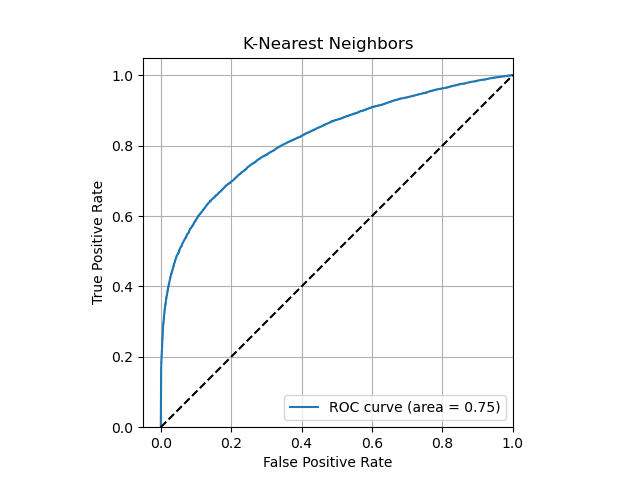
\includegraphics[width=1\linewidth]{docs//assets/individual_roc_curve_K-Nearest Neighbors.png}
    \caption{ROC Curve for K-Nearest Neighbors}
    \label{fig:roc-knn}
\end{figure}

Table~\ref{tab:knn} is the metrics for K-Nearest Neighbors. As a lazy learning algorithm, KNN's precision and AUC is close to decision tree and logistic regression, which is very impressive.

\begin{table}
\centering
\begin{tabular}{|c|c|c|c|c|c|c}
\hline
\textbf{Precision} & \textbf{Recall} & \textbf{Specificity} & \textbf{F1 Score} & \textbf{AUC} & \textbf{Confusion Matrix} \\
\hline
0.835 & 0.620 & 0.878 & 0.711 & 0.749 & $\left(\begin{array}{cc} 14089 & 1963 \\ 6104 & 9947 \end{array}\right)$ \\ 
\hline
\end{tabular}
\caption{Metrics for K-Nearest Neighbors}
\label{tab:knn}
\end{table}

Additionally, elbow method is used to find the optimal K. Figure~\ref{fig:knn-elbow} shows the proceduire of this approach. When k is 27, the plot reaches the knee of the curve, which explains the optimal k found in the grid search.

\begin{figure}
    \centering
    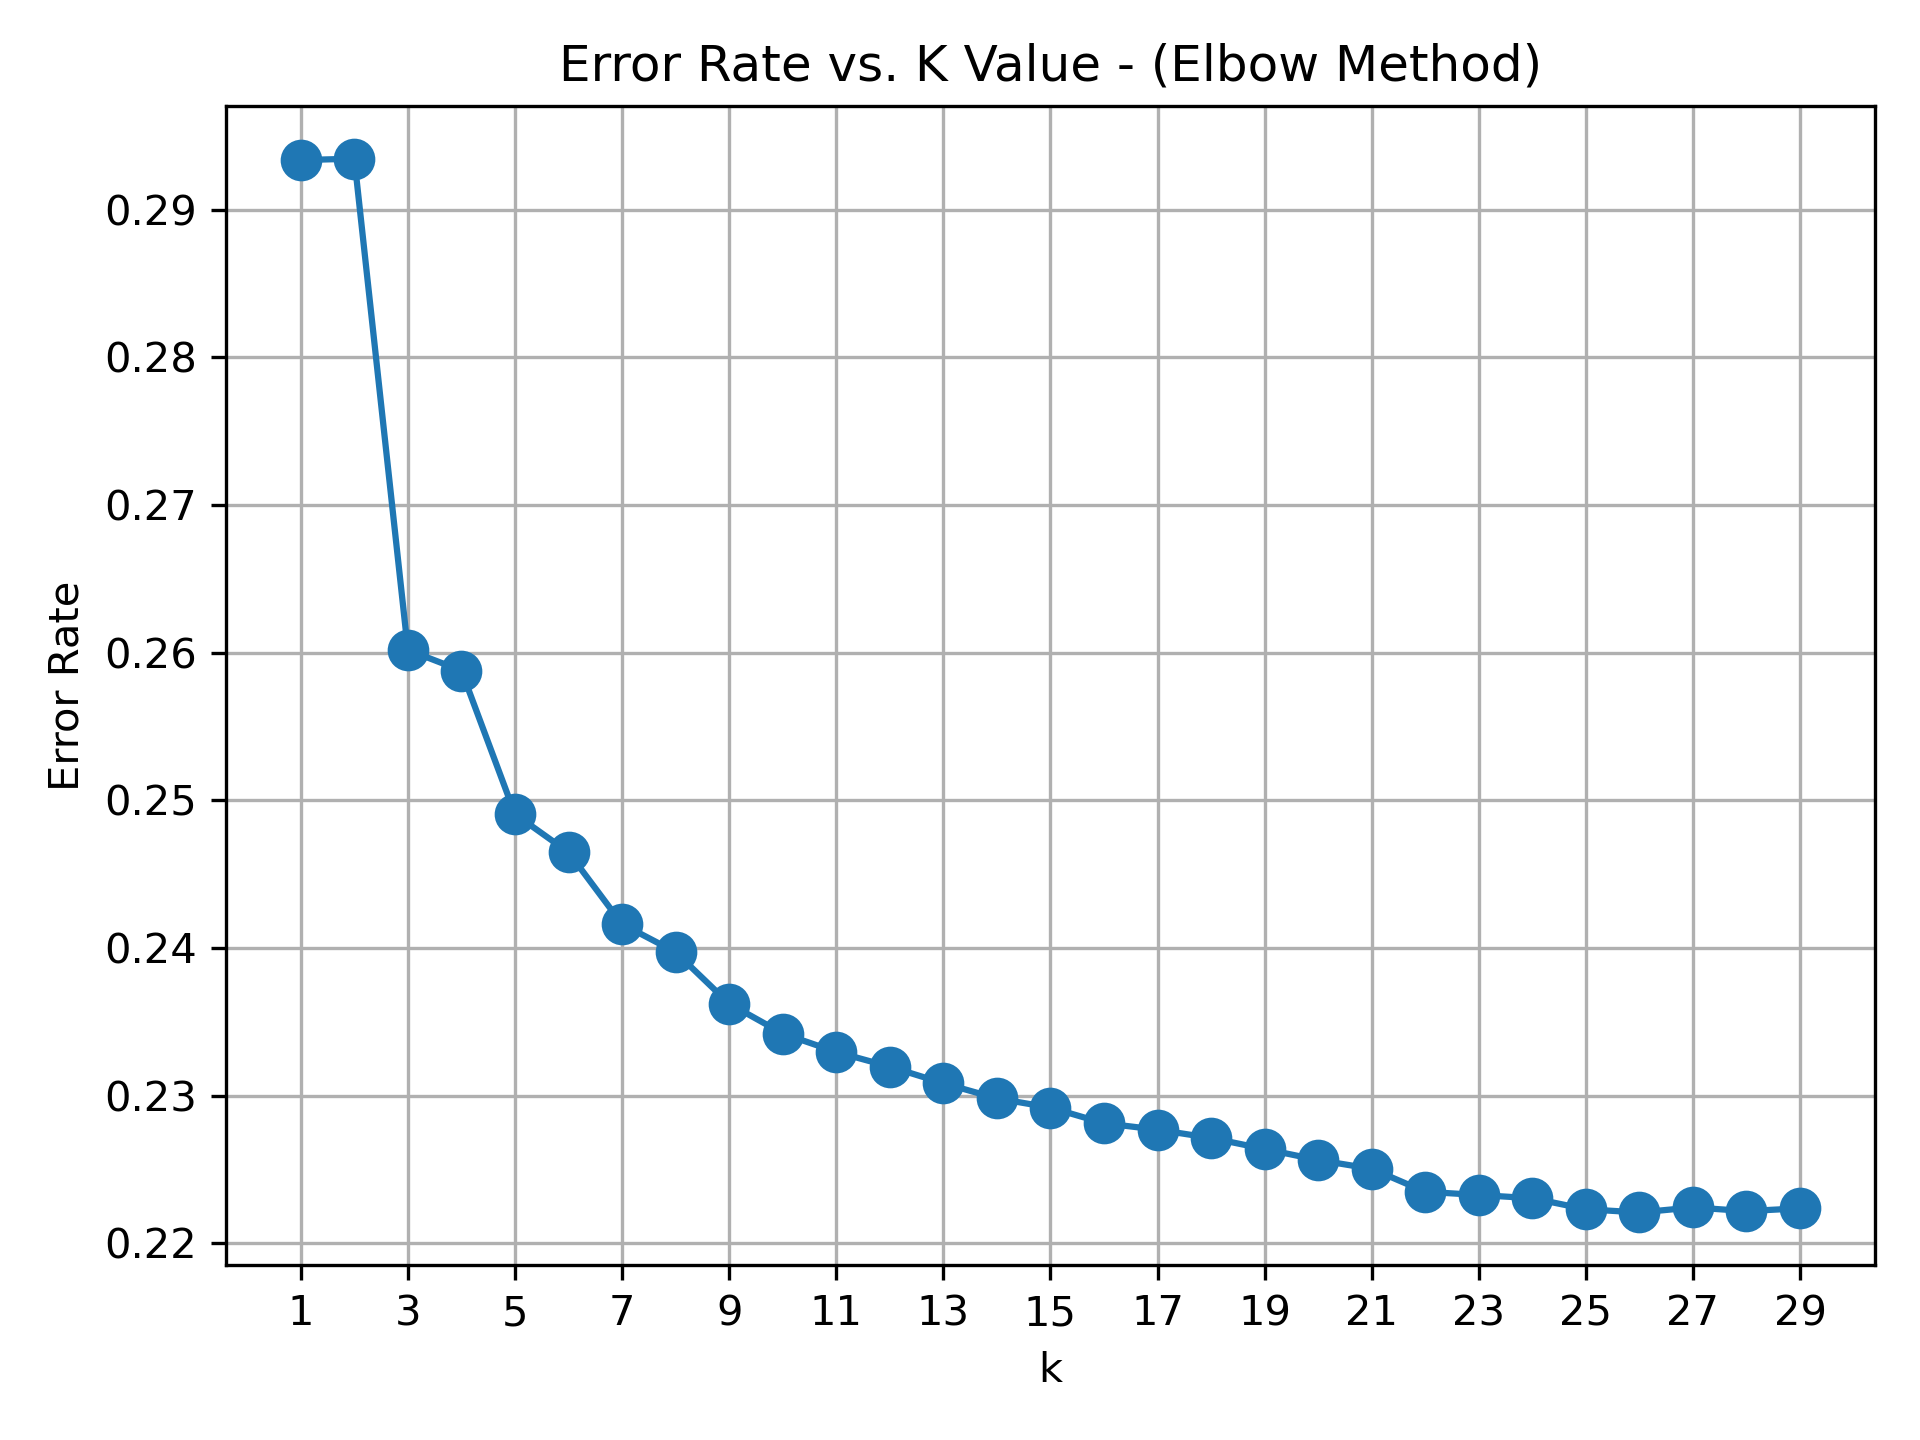
\includegraphics[width=1\linewidth]{docs//assets/elbow_method_knn.png}
    \caption{KNN- Elbow Method Approach to Best K}
    \label{fig:knn-elbow}
\end{figure}


\subsection{Support Vector Machine}

Support Vector Machines (SVM) are a set of supervised learning methods used for classification, regression and outliers detection. In this case, \texttt{sklearn.svm.SVC} is used for classification. The grid search of hyper parameters is the kernel function as shown in table~\ref{tab:parameters-svm}. \textit{Kernel Function generally transforms the training set of data so that a non-linear decision surface is able to transform to a linear equation in a higher number of dimension spaces}\cite{geeksforgeeks_kernel_svm}. 

\begin{table}[h]
\centering
\begin{tabular}{|l|r|}
\hline
\textbf{Parameter} & \textbf{Values}        \\ \hline
kernel             & rbf, linear, poly      \\ \hline
\end{tabular}
\caption{Parameter Candidates for Support Vector Machine}
\label{tab:parameters-svm}
\end{table}

The best parameters for this classifier is rbf kernel as shown in the console:

\begin{verbatim}
Best parameters set found on development set:
{'kernel': 'rbf'}
\end{verbatim}

Figure~\ref{fig:roc-svm} shows the ROC curve of Support Vector Machine classifier, the model obtained an AUC of \textbf{0.79}, comparatively a good fit.

\begin{figure}
    \centering
    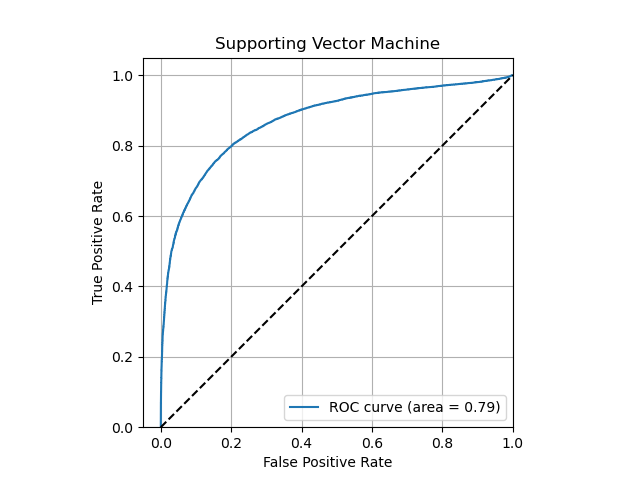
\includegraphics[width=1\linewidth]{docs//assets/individual_roc_curve_Supporting Vector Machine.png}
    \caption{ROC Curve for Support Vector Machine}
    \label{fig:roc-svm}
\end{figure}

Table~\ref{tab:svm} is the metrics for Support Vector Machine. The specificity is relatively high, but the difference between specificity and recall is large. Meaning that the model performs well in avoiding \textit{false alarms}.

\begin{table}
\centering
\begin{tabular}{|c|c|c|c|c|c|c}
\hline
\textbf{Precision} & \textbf{Recall} & \textbf{Specificity} & \textbf{F1 Score} & \textbf{AUC} & \textbf{Confusion Matrix} \\
\hline
0.875 & 0.672 & 0.904 & 0.760 & 0.788 & $\left(\begin{array}{cc} 14515 & 1537 \\ 5263 & 10788 \end{array}\right)$ \\ 
\hline
\end{tabular}
\caption{Metrics for Support Vector Machine}
\label{tab:svm}
\end{table}


\subsection{Na\"ive Bayes}

To implement Na\"ive Bayes Classification, \texttt{sklearn.naive\_bayes.GaussianNB} is utilized. Na\"ive Bayes classifier does not have many parameters that can be used in grid search, based on the general approach of the algorithm's nature. Table~\ref{tab:parameters-nb} shows the parameter candidate: var\_smoothing, which is the portion of the largest variance of all features that is added to variances for calculation stability. In other words, this is passed to the Gaussian probability density function, determining the shape of the Gaussian distribution.

\begin{table}[h]
\centering
\begin{tabular}{|l|r|}
\hline
\textbf{Parameter} & \textbf{Values}                         \\ \hline
var\_smoothing     & \(1 \times 10^{-9}\), \(1 \times 10^{-8}\), \(1 \times 10^{-7}\), \(1 \times 10^{-6}\) \\ \hline
\end{tabular}
\caption{Parameter Candidates for Na\"ive Bayes}
\label{tab:parameters-nb}
\end{table}

The best parameters for var\_smoothing is shown in the console, the same as the default value:

\begin{verbatim}
Best parameters set found on development set:
{'var_smoothing': 1e-09}
\end{verbatim}

Figure~\ref{fig:roc-nb} shows the ROC curve of Na\"ive Bayes classifier, the model obtained an AUC of \textbf{0.70}, lower than the previous classifiers.

\begin{figure}
    \centering
    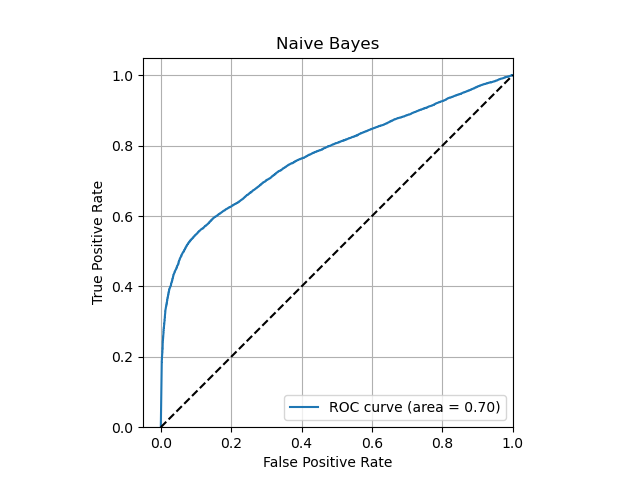
\includegraphics[width=1\linewidth]{docs//assets/individual_roc_curve_Naive Bayes.png}
    \caption{ROC Curve for Na\"ive Bayes}
    \label{fig:roc-nb}
\end{figure}

Table~\ref{tab:nb} is the metrics for Na\"ive Bayes. The F-1 Score is obviously lower than the previous ones, meaning that the model does not provide a good fit in positive or negative predictions compareed to the previous ones whose F1 score is higher than \textbf{0.7}. A possible explaination is that the data did not pass normal test, which makes it a less ideal fit for Na\"ive Bayes.

\begin{table}
\centering
\begin{tabular}{|c|c|c|c|c|c|c}
\hline
\textbf{Precision} & \textbf{Recall} & \textbf{Specificity} & \textbf{F1 Score} & \textbf{AUC} & \textbf{Confusion Matrix} \\
\hline
0.918 & 0.442 & 0.960 & 0.597 & 0.701 & $\left(\begin{array}{cc} 15415 & 637 \\ 8954 & 7097 \end{array}\right)$ \\ 
\hline
\end{tabular}
\caption{Metrics for Na\"ive Bayes}
\label{tab:nb}
\end{table}

\subsection{Random Forest (Bagging)}

The difference between Random Forest here and the one in the previous phase is that random forest here is a classifier, utilized the advantages of ensemble learning and decision tree. It's derived from bagging algorithm. Bagging, short for Bootstrap Aggregating, is a machine learning ensemble technique designed to improve the stability and accuracy of machine learning algorithms. Random Forest is a specific and popular instance of bagging, applied to decision tree classifiers. It introduces an additional layer of randomness compared to standard bagging.

Table~\ref{tab:parameters-rf} shows the tuning parameters used for random forest. \texttt{n\_estimators} is the number of trees in the forest, while \texttt{bootstrap} is whether to use bootstrap. \textit{The bootstrap is a widely applicable and extremely powerful statistical tool that can be used to quantify the uncertainty associated with a given estimator or statistical learning method}\cite{james2023introduction_bootstrap}. In this case, it determines whether the whole dataset is used for each estimator.

\begin{table}[h]
\centering
\begin{tabular}{|l|r|}
\hline
\textbf{Parameter}        & \textbf{Values}         \\ \hline
n\_estimators             & 100, 500                \\ \hline
criterion                 & gini                    \\ \hline
max\_depth                & 4                       \\ \hline
min\_samples\_split       & 2                       \\ \hline
min\_samples\_leaf        & 1                       \\ \hline
max\_features             & 10                      \\ \hline
bootstrap                 & True, False             \\ \hline
\end{tabular}
\caption{Parameter Candidates for Random Forest}
\label{tab:parameters-rf}
\end{table}

The best parameters for var\_smoothing is shown in the console.

\begin{verbatim}
Best parameters set found on development set:
{'bootstrap': True, 'n_estimators': 500}
\end{verbatim}

Figure~\ref{fig:roc-rf} shows the ROC curve of Random Forest classifier, the model obtained an AUC of \textbf{0.79}, comparatively a good fit.

\begin{figure}
    \centering
    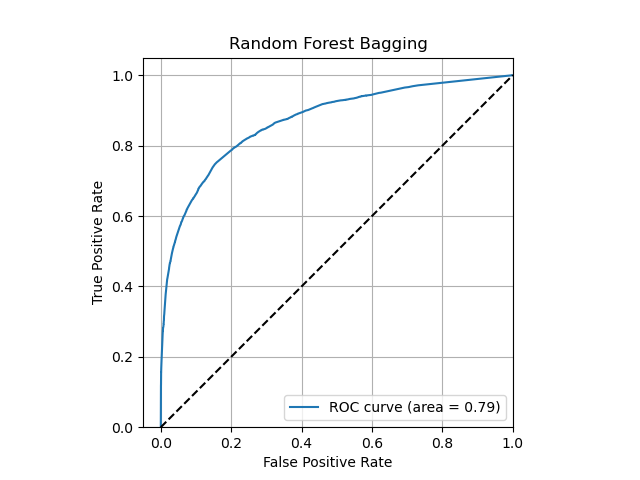
\includegraphics[width=1\linewidth]{docs//assets/individual_roc_curve_Random Forest Bagging.png}
    \caption{ROC Curve for Random Forest}
    \label{fig:roc-rf}
\end{figure}

Table~\ref{tab:rf} is the metrics for Random Forest Classifier. The recall, sensitivity are very close to each other, meaning that the model performs well on both positive and negative predictions.

\begin{table}
\centering
\begin{tabular}{|c|c|c|c|c|c|c}
\hline
\textbf{Precision} & \textbf{Recall} & \textbf{Specificity} & \textbf{F1 Score} & \textbf{AUC} & \textbf{Confusion Matrix} \\
\hline
0.793 & 0.793 & 0.792 & 0.793 & 0.793 & $\left(\begin{array}{cc} 12719 & 3333 \\ 3320 & 12731 \end{array}\right)$ \\ 
\hline
\end{tabular}
\caption{Metrics for Random Forest}
\label{tab:rf}
\end{table}

\subsection{Stacking}

Stacking means the stack of estimators with a final classifier. As described in the document of scikit-learn, stacked generalization consists in stacking the output of individual estimator and use a classifier to compute the final prediction. Stacking allows to use the strength of each individual estimator by using their output as input of a final estimator. In this case, based on a set of classifiers, a final classifier that combined these candidate classifiers will be produced.

Because of the speciality of stacking algorithm, that it does not implement new classifier, but combines other estimators, no grid search on the specific parameter of the model is operated in this part. The Estimators chose to be candidates are as table~\ref{tab:parameters-stacking}.

\begin{table}[h]
\centering
\begin{tabular}{|l|r|}
\hline
\textbf{Parameter}        & \textbf{Values}         \\ \hline
estimators             & SVC, KNN, Naive Bayes                \\ \hline
\end{tabular}
\caption{Parameter Candidates for Stacking}
\label{tab:parameters-stacking}
\end{table}

Figure~\ref{fig:roc-stacking} shows the ROC curve of Stacking classifier, the model obtained an AUC of \textbf{0.80}, which is the \textbf{highest} so far.

\begin{figure}
    \centering
    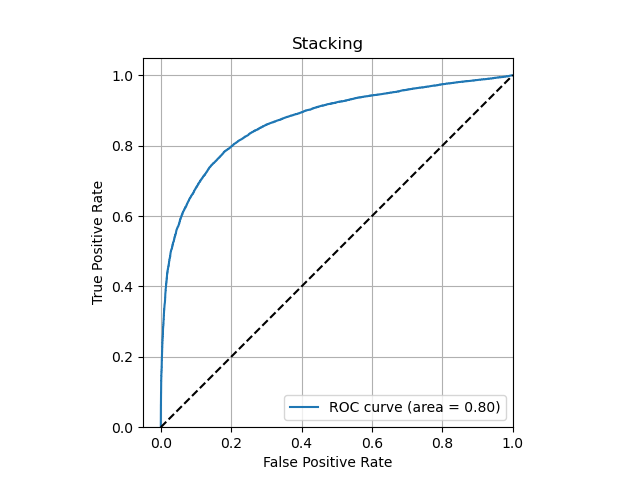
\includegraphics[width=1\linewidth]{docs//assets/individual_roc_curve_Stacking.png}
    \caption{ROC Curve for Stacking}
    \label{fig:roc-stacking}
\end{figure}

Table~\ref{tab:stacking} is the metrics for Stacking Classifier. Compared to random forest, a higher precision is achieved.

\begin{table}
\centering
\begin{tabular}{|c|c|c|c|c|c|c}
\hline
\textbf{Precision} & \textbf{Recall} & \textbf{Specificity} & \textbf{F1 Score} & \textbf{AUC} & \textbf{Confusion Matrix} \\
\hline
0.846 & 0.729 & 0.867 & 0.783 & 0.798 & $\left(\begin{array}{cc} 13921 & 2131 \\ 4346 & 11705 \end{array}\right)$ \\ 
\hline
\end{tabular}
\caption{Metrics for Stacking}
\label{tab:stacking}
\end{table}

\subsection{Boosting}

Boosting is achieved using \texttt{sklearn.ensemble.AdaBoostClassifier}. According to scikit-learn,\textit{ an AdaBoost classifier is a meta-estimator that begins by fitting a classifier on the original dataset and then fits additional copies of the classifier on the same dataset but where the weights of incorrectly classified instances are adjusted such that subsequent classifiers focus more on difficult cases.}

Table~\ref{tab:parameters-boosting} shows the parameter grid for boosting. \texttt{learning\_rate} is weight applied to each classifier at each boosting iteration. A higher learning rate increases the contribution of each classifier. Meaning that there's a trade-off between learning rate and number of estimators.

\begin{table}[h]
\centering
\begin{tabular}{|l|r|}
\hline
\textbf{Parameter}    & \textbf{Values}          \\ \hline
n\_estimators         & 50, 200, 500             \\ \hline
learning\_rate        & 0.1, 0.5, 1.0            \\ \hline
\end{tabular}
\caption{Parameter Candidates for Boosting Model}
\label{tab:parameters-boosting}
\end{table}

The best parameters are shown in the console:

\begin{verbatim}
Best parameters set found on development set:
{'learning_rate': 0.5, 'n_estimators': 200}
\end{verbatim}

Figure~\ref{fig:roc-boosting} shows the ROC curve of boosting classifier, the model obtained an AUC of \textbf{0.80}, which comparatively very high.

\begin{figure}
    \centering
    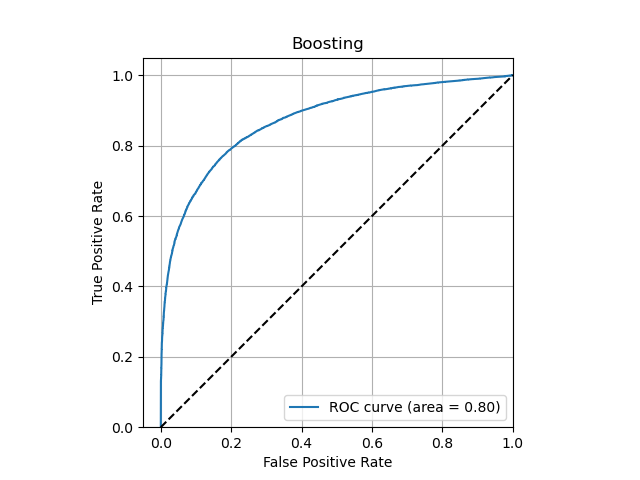
\includegraphics[width=1\linewidth]{docs//assets/individual_roc_curve_Boosting.png}
    \caption{ROC Curve for Boosting}
    \label{fig:roc-boosting}
\end{figure}

Table~\ref{tab:boosting} is the metrics for Boosting Classifier. This classifier does well on nearly all metrics, obtaining a higher precision than random forest.

\begin{table}
\centering
\begin{tabular}{|c|c|c|c|c|c|c}
\hline
\textbf{Precision} & \textbf{Recall} & \textbf{Specificity} & \textbf{F1 Score} & \textbf{AUC} & \textbf{Confusion Matrix} \\
\hline
0.817 & 0.764 & 0.829 & 0.790 & 0.797 & $\left(\begin{array}{cc} 13313 & 2739 \\ 3782 & 12269 \end{array}\right)$ \\ 
\hline
\end{tabular}
\caption{Metrics for Boosting}
\label{tab:boosting}
\end{table}

\subsection{Neural Network}

Neural network is a high-efficiency classifier. In this part the project estimated a multi-layered perceptron neural-network, with grid parameters shown in table~\ref{tab:parameters-neural-network} shows the parameter grid for boosting. \texttt{solver} is the argument to set the optimization algorithm, \texttt{activation} is for introducing non-linearity of the mode. The tuning option is the hidden layer sizes: (100,) means one hidden layer with 100 hidden units and (100, 100) means two hidden layers with 100 hidden units each.

\begin{table}[h]
\centering
\begin{tabular}{|l|r|}
\hline
\textbf{Parameter}        & \textbf{Values}                \\ \hline
hidden\_layer\_sizes      & (100,), (100, 100)             \\ \hline
activation                & relu                           \\ \hline
solver                    & adam                           \\ \hline
learning\_rate            & constant                       \\ \hline
\end{tabular}
\caption{Parameter Candidates for Neural Network}
\label{tab:parameters-neural-network}
\end{table}

The best parameters are shown in the console as following. One hidden layer performs better for this dataset.

\begin{verbatim}
Best parameters set found on development set:
{'activation': 'relu', 'hidden_layer_sizes': (100,), 
'learning_rate': 'constant', 'solver': 'adam'}
\end{verbatim}

Figure~\ref{fig:roc-nn} shows the ROC curve of boosting classifier, the model obtained an AUC of \textbf{0.80}. It's one of the best models of the classifiers discussed in this section.

\begin{figure}
    \centering
    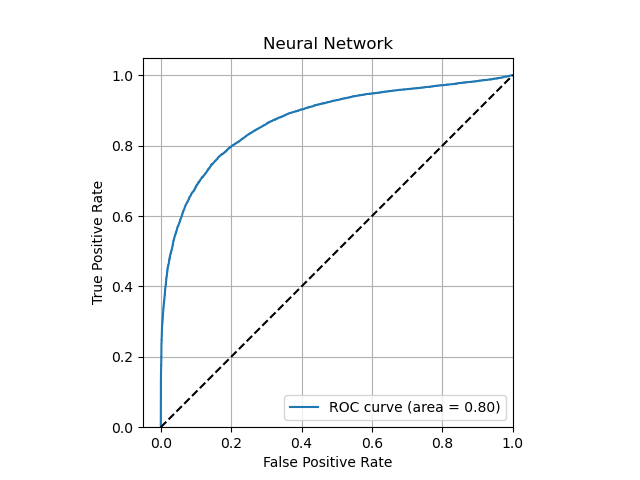
\includegraphics[width=1\linewidth]{docs//assets/individual_roc_curve_Neural Network.png}
    \caption{ROC Curve for Neural Network}
    \label{fig:roc-nn}
\end{figure}

Table~\ref{tab:nn} is the metrics for Neural Network Classifier. It obtains a high precision and a high F1 score.

\begin{table}
\centering
\begin{tabular}{|c|c|c|c|c|c|c}
\hline
\textbf{Precision} & \textbf{Recall} & \textbf{Specificity} & \textbf{F1 Score} & \textbf{AUC} & \textbf{Confusion Matrix} \\
\hline
0.824 & 0.767 & 0.836 & 0.794 & 0.802 & $\left(\begin{array}{cc} 13313 & 2739 \\ 3782 & 12269 \end{array}\right)$ \\ 
\hline
\end{tabular}
\caption{Metrics for Neural Network}
\label{tab:nn}
\end{table}

\subsection{Conclusion}

The metrics of all of the classifiers are shown in table~\ref{tab:master-table}. \

In conclusion, the extensive classification analysis conducted on various machine learning classifiers demonstrates a range of performance metrics, each with its unique strengths and weaknesses. The Decision Tree classifiers, both pre-pruning and post-pruning, showed balanced performance across precision, recall, specificity, F1 score, and AUC, indicating their effectiveness in handling both positive and negative classes. However, the Logistic Regression model excelled in specificity, suggesting its strength in reducing false positives.

The K-Nearest Neighbors classifier, although a lazy learning algorithm, presented impressive precision and AUC, close to those of more complex models. The Support Vector Machine, with its high precision and specificity, proved to be excellent at avoiding false alarms but less effective in recall.

Naïve Bayes, despite having the highest precision, lagged in recall and F1 score, possibly due to the data's non-normal distribution. In contrast, the Random Forest Bagging method achieved a remarkable balance across all metrics, making it a robust choice.

Stacking, which combines multiple estimators, emerged with the highest AUC, indicating its superior predictive power. Similarly, the Boosting model displayed high scores across all metrics, particularly excelling in precision and F1 score. Finally, the Neural Network, with one of the best AUCs, showed high precision and F1 score, affirming its efficiency as a classifier.

Overall, the best classifier recommended for this dataset is \textbf{Neural Network Classifier}. It balances all metrics and has the highest AUC and F1 score without compromising precision or recall. In figure~\ref{fig:master-roc} shows the ROC of all the classifiers discussed, from which no obvious difference is observed except for Na\"ive Bayes Classifier. The dataset demonstrates a good fit of classification model compared to regression models.

\begin{table}[]
    \scriptsize
    \centering
    \begin{tabular}{|r|c|c|c|c|c|c|}
    \hline
        \textbf{Classifier} & \textbf{Precision} & \textbf{Recall} & \textbf{Specificity} & \textbf{F1 Score} & \textbf{AUC} & \textbf{Confusion Matrix} \\
        \hline
        Decision Tree Pre-pruning & 0.804 & 0.770 & 0.812 & 0.786 & 0.791 & $\left(\begin{array}{cc} 13032 & 3020 \\ 3699 & 12352 \end{array}\right)$ \\
        Decision Tree Post-pruning & 0.812 & 0.727 & 0.831 & 0.767 & 0.779 & \begin{array}{cc} 13345 & 2707 \\ 4381 & 11670 \end{array} \\
        Logistic Regression & 0.864 & 0.641 & 0.899 & 0.736 & 0.770 & $\left(\begin{array}{cc} 14437 & 1615 \\ 5756 & 10295 \end{array}\right)$ \\
        K-Nearest Neighbors & 0.835 & 0.620 & 0.878 & 0.711 & 0.749 & \begin{array}{cc} 14089 & 1963 \\ 6104 & 9947 \end{array} \\
        Support Vector Machine & 0.875 & 0.672 & 0.904 & 0.760 & 0.788 & $\left(\begin{array}{cc} 14515 & 1537 \\ 5263 & 10788 \end{array}\right)$ \\
        Naive Bayes & \textbf{0.918} & \underline{0.442} & \textbf{0.960} & \underline{0.597} & \underline{0.701} & \begin{array}{cc} 15415 & 637 \\ 8954 & 7097 \end{array} \\
        Random Forest Bagging & \underline{0.793} & \textbf{0.793} & \underline{0.792} & 0.793 & 0.793 & $\left(\begin{array}{cc} 12719 & 3333 \\ 3320 & 12731 \end{array}\right)$ \\
        Stacking & 0.846 & 0.729 & 0.867 & 0.783 & 0.798 & \begin{array}{cc} 13921 & 2131 \\ 4346 & 11705 \end{array} \\
        Boosting & 0.817 & 0.764 & 0.829 & 0.790 & 0.797 & $\left(\begin{array}{cc} 13313 & 2739 \\ 3782 & 12269 \end{array}\right)$ \\
        Neural Network & 0.824 & 0.767 & 0.836 & \textbf{0.794} & \textbf{0.802} & \begin{array}{cc} 13422 & 2630 \\ 3740 & 12311 \end{array} \\
        \hline
\end{tabular}
    \caption{Comparison of Classifiers}
    \label{tab:master-table}
\end{table}

\begin{figure}
    \centering
    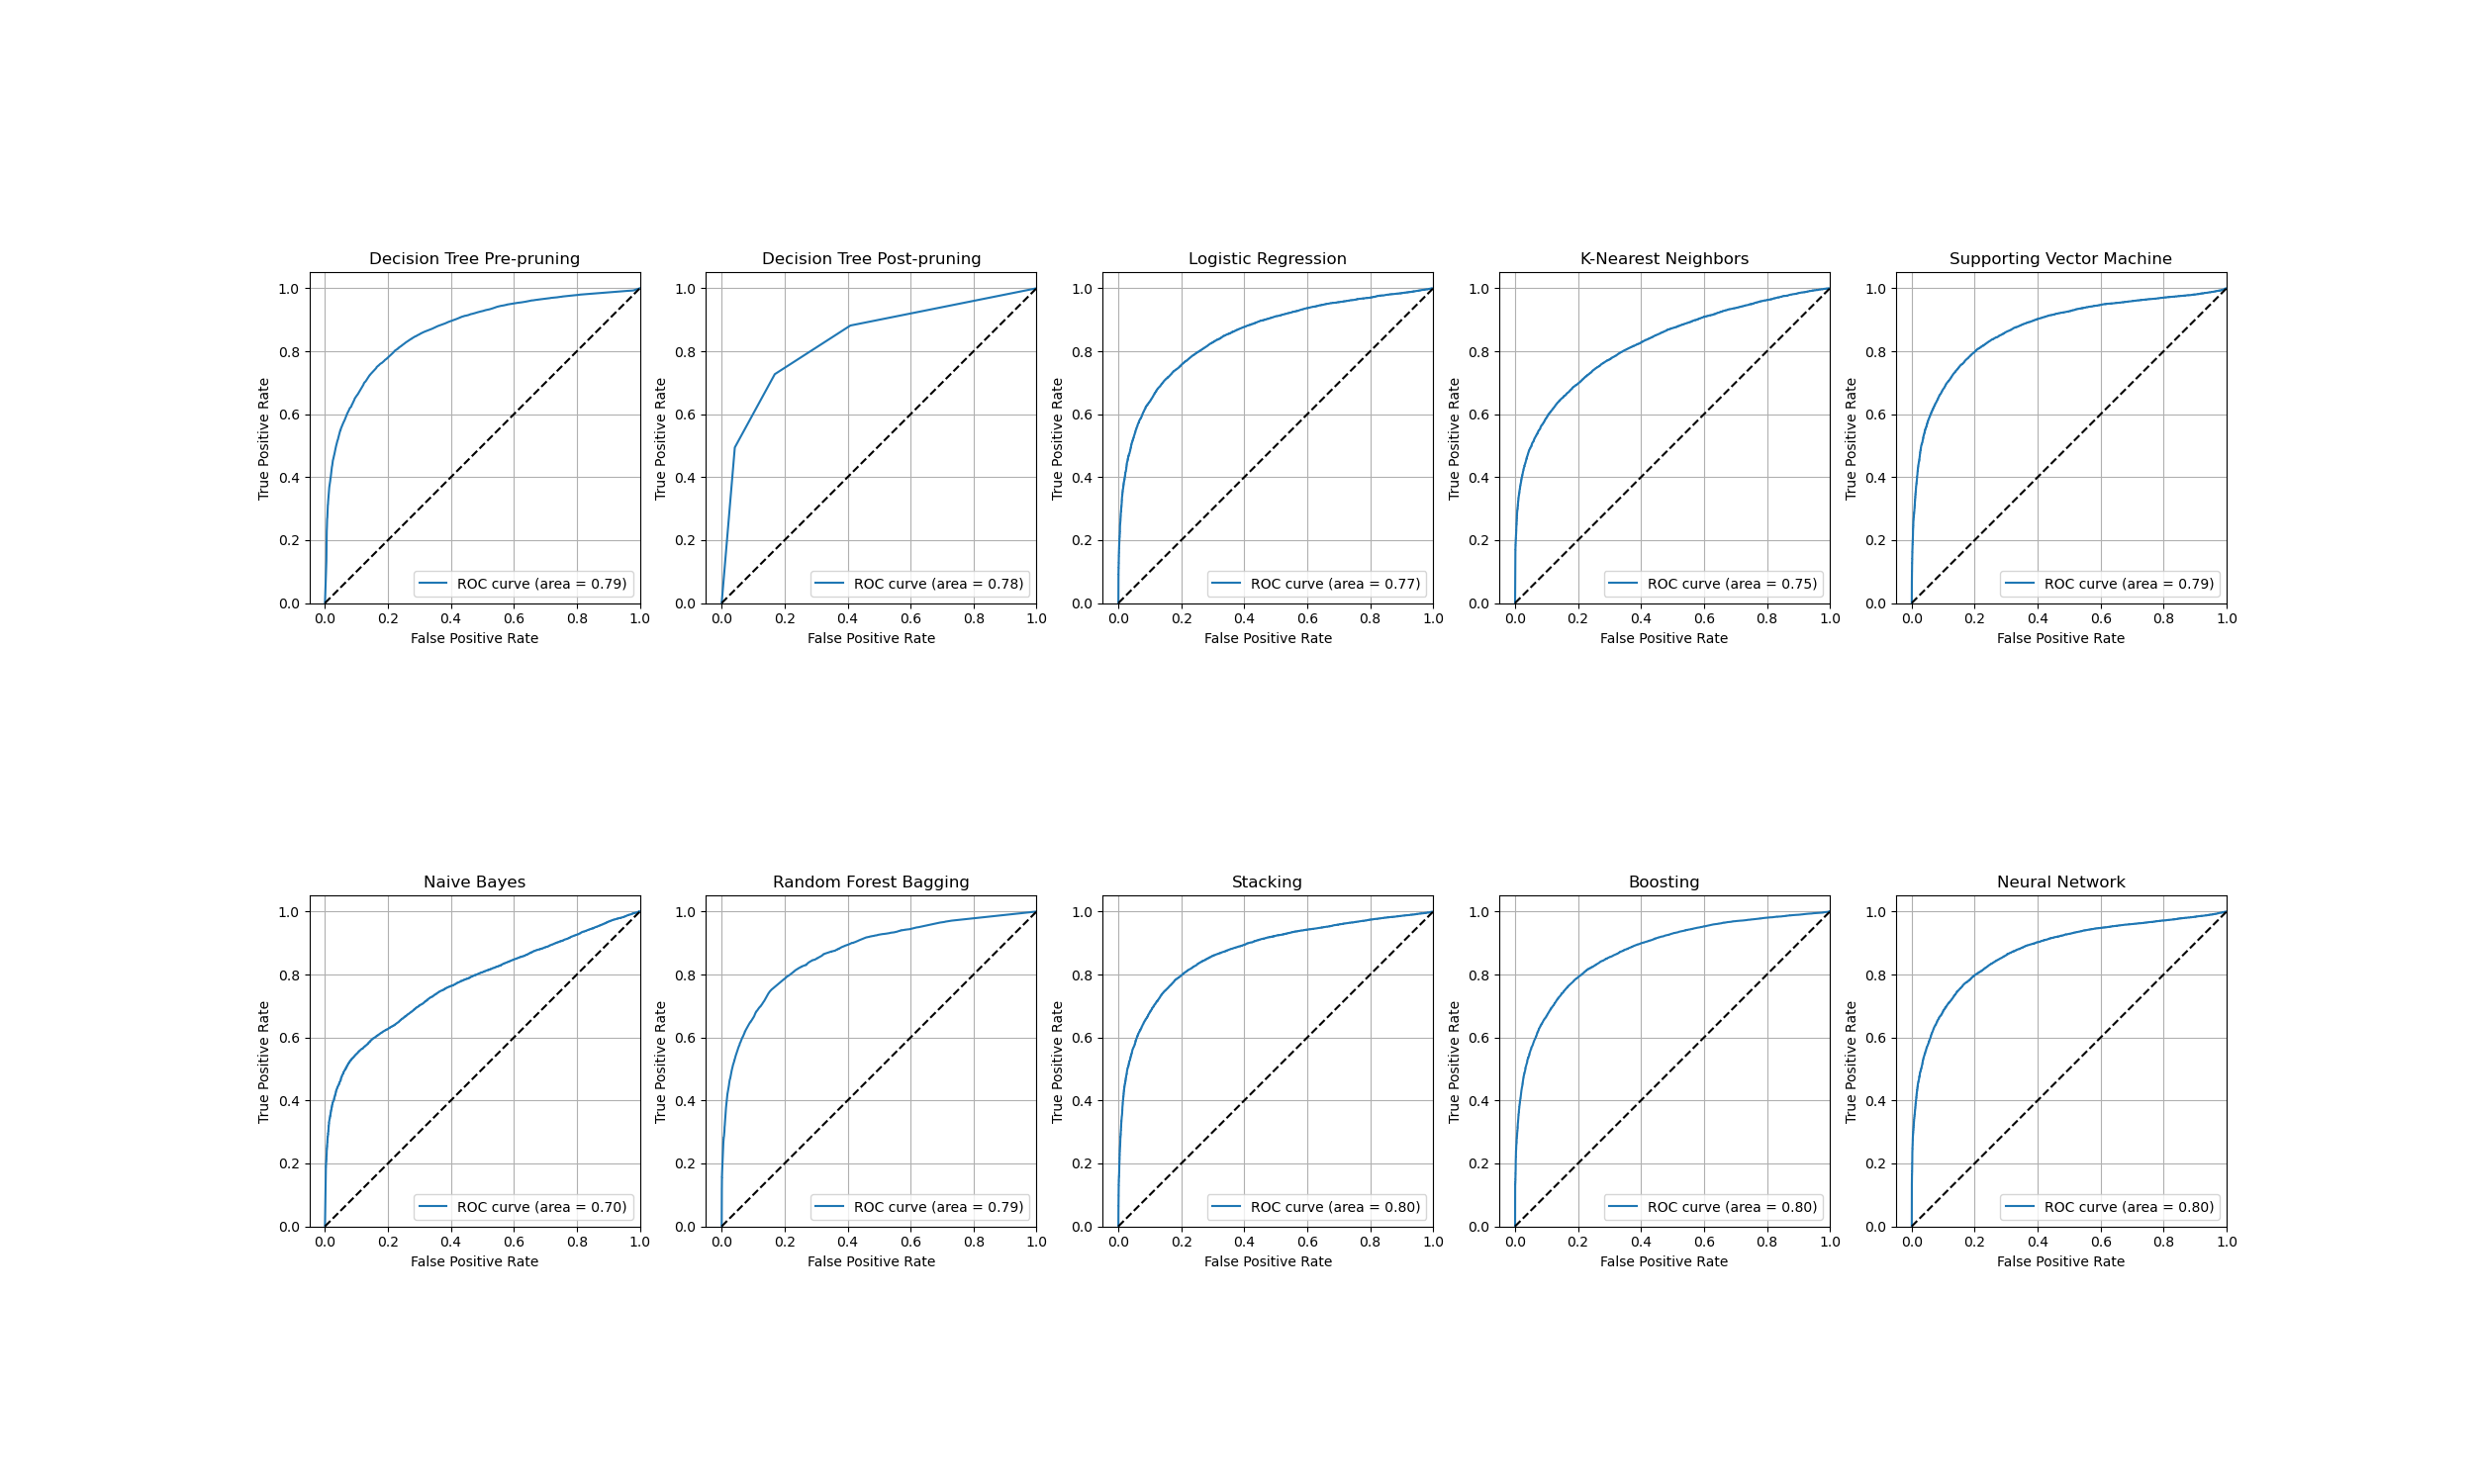
\includegraphics[width=1\linewidth]{master_roc_curve.png}
    \caption{ROC of Classifiers}
    \label{fig:master-roc}
\end{figure}

